\section{Analysis of Covariance (ANCOVA)}\label{ANCOVA}
In Section \ref{sec:Hyp.Testing}, we looked at the effectiveness of new teaching method by assigning each group to a specific treatment and comparing the mean test scores. A crucial assumption for that model is that subjects in each group have \textbf{similar background knowledge} about statistics prior to the three week lectures. \par If this assumption is wrong, however, we may be making incorrect decisions based on the model. Even if each group had similar background knowledge \textit{on average}, there may be large variability from person-to-person, masking the true treatment effect.

\subsection{Paired Comparison}
One way to avoid such \textbf{subject-to-subject variability} is to administer both treatments to each individual,  and then compare treatment effects by looking at the \textbf{difference in the outcomes}. \newl For instance, if a grocery chain is interested in measuring the effectiveness of two advertising campaigns, it could be reasonable to assume that there is a large variability in total sales, as well as popular items sold, at each store. \par It may then be preferable to run both campaigns in each store and analyse the resulting data rather than to split the stores into two groups (in each of which a different advertising campaign is run) and then to compare the mean outcomes in the two groups. 
\newl Formally, let $X_{i,1}$ denote the total sales with campaign $A$ and $X_{i,2}$ the total sales with campaign $B$. The quantity of interest is the \textbf{difference} $D_{i}=X_{i,1}-X_{i,2}$ for each store $i=1,\ldots,N$. \par Assuming that the differences $D_{i}$ follow an {i.i.d.} normal distribution with mean $\delta$ and variance $\sigma^{2}_{d}$, then we  test for $$H_{0}: \delta=0\quad\mbox{against}\quad H_{1}: \delta \neq 0$$  using the test statistic $$t_0=\sqrt{N}\frac{\bar{D}}{s_{d}},$$ which follows a Student's $t$ distribution with  $N-1$ degrees of freedom; thus we reject $H_{0}$ if the observed test statistic $t_{0}$ has $p$-value less than the significance level $\alpha/2$.

\begin{figure}[!t]
\centering
  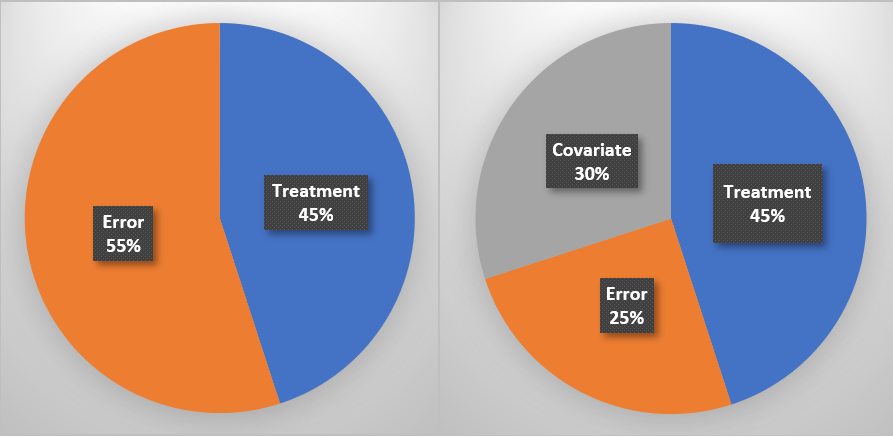
\includegraphics[width=0.95\linewidth]{Images/testA14.png}
  \caption[\small Breakdown of variability for ANOVA and ANCOVA]{\small Breakdown of variability for ANOVA and ANCOVA.}
  \label{fig:testA14}\hrule
\end{figure}
\afterpage{\FloatBarrier}
\subsection{Analysis of Covariance (ANCOVA)}
ANOVA compares multiple group means and tests whether any of the group means differ from the rest, by breaking down the total variability into a treatment (explainable) variability component and an error (unexplained) variability component, and building a ratio $F_0$ to determine whether or not to reject $H_{0}$. \par \textbf{Analysis of covariance} (ANCOVA) introduces \textbf{concomitant variables} (or \textbf{covariates}) to the ANOVA model, splitting the total variability into 3 components: $\text{SS}_{\textrm{treat}}$, $\text{SS}_{\textrm{con}}$, and $\text{SS}_{\textrm{e}}$, aiming to reduce error variability. The choice of covariates is thus crucial in running a successful ANCOVA.
\newl In order to be useful, a concomitant variable must be related to response variable in some way, otherwise it not only fails to reduce error variability, but it also increases the model complexity: 
\begin{itemize}[noitemsep]
\item in the teaching method example, we could consider administering a pre-study test to measure the \textbf{prior knowledge level} of each participant and use this score as a concomitant variable;
\item in the advertising campaign example, we could have used the \textbf{previous month's sales} as a covariate; 
\item in medical studies, we could use the \textbf{age} and \textbf{weight} of subjects, say.\end{itemize} Importantly, concomitant variables should not be affected by treatments. As an example, suppose that the patients in a medical study were asked:  \begin{quote} How strongly do you believe that you were given actual medication rather than a placebo?
\end{quote} If the treatment is indeed effective, then a participant's response to this question could be \textbf{markedly different} in the treatment group than in the  placebo group.\footnote{The medication may have strong side-effects which cannot be ignored.} This means that true treatment effect may be masked by concomitant variable due to unequal effects on treatment groups.
\newl Note that \textbf{qualitative covariates} (such as gender, say) are not part of the ANCOVA framework  -- indeed, such covariates create new ANOVA treatment groups instead. \newpage\noindent Figure \ref{fig:testA14} shows a potential breakdown of the total variability when moving from an ANOVA to an ANCOVA model -- the error variability is further split into a \textbf{pure error}  and a \textbf{covariate} component, while the \textbf{treatment} variability remains unchanged.

\subsection{ANCOVA Model and Assumptions}
Suppose that we are testing the effect of $p$ treatments, with $N_{j}$ subjects in each group. Then the ANCOVA model takes the form
\begin{equation}\label{eq:ANCOVA}
    y_{i,j}=\mu+\tau_{j}+\gamma (x_{i,j}-\bar{x})+\varepsilon_{i,j}
\end{equation}
where 
\begin{itemize}[noitemsep]
    \item $y_{i,j}$ is the response of the $i^{\text{th}}$ subject in the $j^{\text{th}}$ treatment group;
    \item $\mu$ is the overall mean;
    \item $\tau_{j}$ is the $j^{\text{th}}$ treatment effect, subject to a constraint $$\sum_{j=1}^{p}\tau_{j}=0;$$
    \item $\gamma$ is the coefficient for the \textbf{covariate effect};
    \item $(x_{i,j}-\bar{x})$ is the covariate value of the $i^{\text{th}}$ subject in the $j^{\text{th}}$ treatment group, adjusted by the mean, and
    \item $\varepsilon_{i,j}$ is the error of $i^{\text{th}}$ subject in the $j^{\text{th}}$ treatment group.
\end{itemize}
Additionally, four assumptions must be satisfied:
\begin{itemize}[noitemsep]
    \item \textbf{independence and normality of residuals} -- the residuals follow an ${i.i.d.}$ normal distribution with mean of $0$ and variance $\sigma^{2}_{\varepsilon}$;
    \item \textbf{homogeneity of residual variances} -- the variance of the residuals is uniform across treatment groups;
    \item \textbf{homogeneity of regression slopes} -- the regression effect (slope) is uniform across treatment groups, and
    \item \textbf{linearity of regression} -- the regression relationship between the response and the covariate is linear.
\end{itemize}
The first of these assumptions can be tested with the help of a QQ-plot and a scatter-plot of residuals vs.\@ fitted values, while the second may use the Bartlett or the Levene test. The final assumption is not as crucial as the other three assumptions. Various remedial methods can be applied should any of these assumptions fail.  
\newl The third assumption, however, is \textbf{crucial} to the ANCOVA model; it can be tested with the \textbf{equal slope test}, which requires an ANCOVA regression on equation (\ref{eq:ANCOVA}) with an additional interaction term $x \times \tau$. \par If the interaction is not significant, the third assumption is satisfied. In the event that the interaction term is statistically significant, a different approach (e.g. moderated regression analysis, mediation analysis) is required since using the original ANCOVA model is not prescribed. \newl An in-depth application of an ANCOVA model is highlighted in Section \ref{sec:CCNM}.

%%%%%%%%%%%%%%%%%%%%%%%%%%%%%%%Section 10%%%%%%%%%%%%%%%%%%%%%%%%%%%%%%%%%%% 

